% This file contains the header data for all assignment files
\documentclass[onecolumn, 11pt]{article}

\usepackage{bbold}   %Get fancy double struck math notation for sets
\usepackage{cite}
\usepackage{cleveref}
\usepackage{color}
\usepackage{courier}   %Have code written out nicely
\usepackage{float}
\usepackage[top=1in, bottom=1in, left=1in, right=1in]{geometry}
\usepackage{graphicx} % handles graphics and figures
\usepackage{hyperref}
\usepackage{listings}
\usepackage{mathtools,bm}
\usepackage{multicol}

\catcode`\^^M=10      %  Makes blank lines meaningless, force use of \par

\definecolor{magenta}{rgb}{0.8,0.0,1.0}
\definecolor{darkGreen}{rgb}{0.0,0.4,0.0}
\definecolor{blue}{rgb}{0.0, 0.0, 0.9}
\definecolor{purple}{rgb}{0.7, 0.0, 0.7}
\definecolor{darkGreen}{rgb}{0.0,0.4,0.0}

\newcommand{\quotes}[1]{``#1''}
\newcommand{\todo}[1]{{\color{magenta}\par {[{\bf ToDo: } {\em #1}} ] \\    }}

\newcommand{\norm}[1]{\left\lVert#1\right\rVert}

%%%%%%%%%%%%%%%%%%%%%%%%%%%%%%%%%%%%%%%%%%%%%%%%%%%%%%%%%%%%%%%%%%%%%%%%%%%%%%%
% NOTE:
%
% The following block of commands is used to format Matlab code blocks for the
% listings package. This block of code is based on two examples:
%  -->   https://gist.github.com/eyliu/120689
%  -->   http://links.tedpavlic.com/ascii/homework_new_tex.ascii
%
% Import file block using:
%   \lstinputlisting{fileName.m}
%
\lstloadlanguages{Matlab}
%
\lstset{language=Matlab,                        % Use MATLAB
        frame=single,                           % Single frame around code
        basicstyle=\small\ttfamily,             % Use small true type font
        keywordstyle=[1]\color{blue}\bfseries,  % MATLAB functions bold and blue
        keywordstyle=[2]\color{purple},         % MATLAB function arguments purple
        keywordstyle=[3]\color{blue}\underbar,  % User functions underlined and blue
        identifierstyle=,                       % Nothing special about identifiers
                                                % Comments small dark green courier
        commentstyle=\usefont{T1}{pcr}{m}{sl}\color{darkGreen}\small,
        stringstyle=\color{darkGreen},            % Strings are purple
        showstringspaces=false,                 % Don't put marks in string spaces
        tabsize=4,                              % 4 spaces per tab
        %
        %%% Put standard MATLAB functions not included in the default
        %%% language here
        morekeywords={xlim,ylim,var,alpha,factorial,poissrnd,normpdf,normcdf},
        %
        %%% Put MATLAB function parameters here
        morekeywords=[2]{on, off, interp},
        %
        %%% Put user defined functions here
        morekeywords=[3]{FindESS, homework_example},
        %
        morecomment=[l][\color{blue}]{...},     % Line continuation (...) like blue comment
        numbers=left,                           % Line numbers on left
        firstnumber=1,                          % Line numbers start with line 1
        numberstyle=\tiny\color{blue},          % Line numbers are blue
        stepnumber=5                            % Line numbers go in steps of 5
        }
%
%%%%%%%%%%%%%%%%%%%%%%%%%%%%%%%%%%%%%%%%%%%%%%%%%%%%%%%%%%%%%%%%%%%%%%%%%%%%%%%


% Special settings for matlab code on exam
\lstset{morekeywords={runSloppySimulation,runSimBadly,simStepMidpointMethod}}

\newcommand{\scoreMark}[0]{$\rule{1.5cm}{0.15mm}$ / $\rule{1.5cm}{0.15mm}$}

%========================================================================
\title{ME 149:  Midterm Exam Solution}
\date{March 15  ---  Start: 6:00pm  ---  End: 7:15pm}
\author{Optimal Control for Robotics}
%========================================================================
\begin{document}
\maketitle

\begin{abstract*}
No calculators, notes, books, or computers allowed. Total time:  75 minutes.
\end{abstract*}
%=================================================

\vspace{1em}

\section*{Student Name:    SOLUTION}

\vspace{1em}

\section*{How to optimize your score?}

\begin{itemize}  \setlength\itemsep{0.1em} \setlength\itemindent{18pt}
  \item Be neat and well organized
  \item For longer problems, show intermediate steps and box your
  \fbox { \parbox{3em}{answer} }
  \item If you need extra space...
        use the back of the page,
        the final (blank) page of the exam,
        or ask for more paper.
        Clearly indicate where the extra work is.
  \item Define all variables that you use and state any assumptions that you make.
\end{itemize}


\vspace{1em}

\section*{Score:  \scoreMark}
\vspace{1em}
\begin{large}
\begin{multicols}{2}
\begin{enumerate}  \setlength\itemsep{1.1em} \setlength\itemindent{36pt}
\item \scoreMark
\item \scoreMark
\item \scoreMark
\item \scoreMark
\item \scoreMark
\item \scoreMark
\item \scoreMark
\item \scoreMark
\item \scoreMark
\end{enumerate}
\end{multicols}
\end{large}


% Force enumerated lists to use letters
\renewcommand{\theenumi}{\Alph{enumi}}

%~~~~~~~~~~~~~~~~~~~~~~~~~~~~~~~~~~~~~~~~~~~~~~~~~~~~~~~~~~~~~~~~~~~~~~~~~~~~~

\pagebreak
\section{Newton's Method}

\begin{enumerate}
  \item Suppose that you want to solve the scalar nonlinear equation $f(x) = 0$. \\
        The current estimate of the root is given by $x_k$
        and the next estimate of the root is given by $x_{k+1}$.
        Derive the Newton-Rhapson update that computes $x_{k+1}$ given $x_k$.
        \\[1em]

        \begin{align*}

          &f(x) = f(x_0) + \Delta x \cdot f'(x_0) + \mathcal{O}(\Delta x^2)
          \quad &\quad
          &\text{Taylor series approx. for $f(x)$ near $x_0$} \\[1em]

          &f(x) \approx f(x_0) + \Delta x \cdot f'(x_0)
          \quad &\quad
          &\text{Let high order terms $\mathcal{O}(\Delta x^2) \to 0$} \\[1em]

          &0 = f(x_0) + \Delta x \cdot f'(x_0)
          \quad &\quad
          &\text{Set linear approximation equal to zero} \\[1em]

          &0 = f(x_k) + (x_{k+1} - x_k) \cdot f'(x_k)
          \quad &\quad
          &\text{Replace $x_0$ with $x_k$ and $\Delta x$ with $x_{k+1} - x_k$ } \\[1em]

          &x_{k+1} = x_k - \frac{f(x_k)}{f'(x_k)}
          \quad &\quad
          &\text{Solve for $x_{k+1}$ } \\[1em]

        \end{align*}


  \item What is the difference between the Newton--Rhapson
        and the secant methods for scalar root finding?
        In what situation would you prefer one to the other?
        \\[2em]

        \textit{Both methods work by computing the root of a local linear
        approximation of the nonlinear function. The two differ in the way that
        this linear approximation is constructed. Newton's method uses the
        analytic derivative of the function to construct the linear model.
        The secant method uses the function value at the current and previous
        point to construct the linear model --- it uses a finite difference
        equation.}
        \\[2em]

        \textit{The Newton--Rhapson method for root finding is prefered to the
        secant method when the analytic derivative is known:
        it will converge more rapidly than the secant method.
        The secant method is used when the analytic derivative is unknown.}

  \pagebreak
  \item Draw a figure that clearly demonstrates a situation in which
        Newton's method will fail to converge to a root of the function.
        Why does the Newton--Rhapson method fail in this situation?
        \\[2em]

        \textit{The Newton--Rhapson method for root finding can fail to
        converge in a variety of situations. One example is shown in
        Figure \ref{fig:newtonRhapsonStability}. Both the top and bottom
        sub-plots show the method applied to the hyperbolic tangent function.
        A small change in the initialization makes the difference between
        convergence (top plot) and divergence (bottom plot).
        When diverging, each iteration moves the current approximation of the
        root farther from the true root, until the approximation (in this case)
        reaches infinity.

        The method will also fail in situations where there is no root, or
        where there is a local extremum where the function does not cross
        the x-axis. In either situation the solver will get stuck in a limit
        cycle around the extremum.

        Finally, if the solver every finds a point where the slope of the
        function is tiny (or zero) then it will extrapolate to near-infinity,
        which almost always will cause the method to fail.

        One key insight is that the convergence of the Newton--Rhapson method
        depends entirely on the initial condition! You can typically find an
        initial guess that will converge to the root, although it might be
        very difficult to do so.}

  \begin{figure}[ht]
  	\centering
    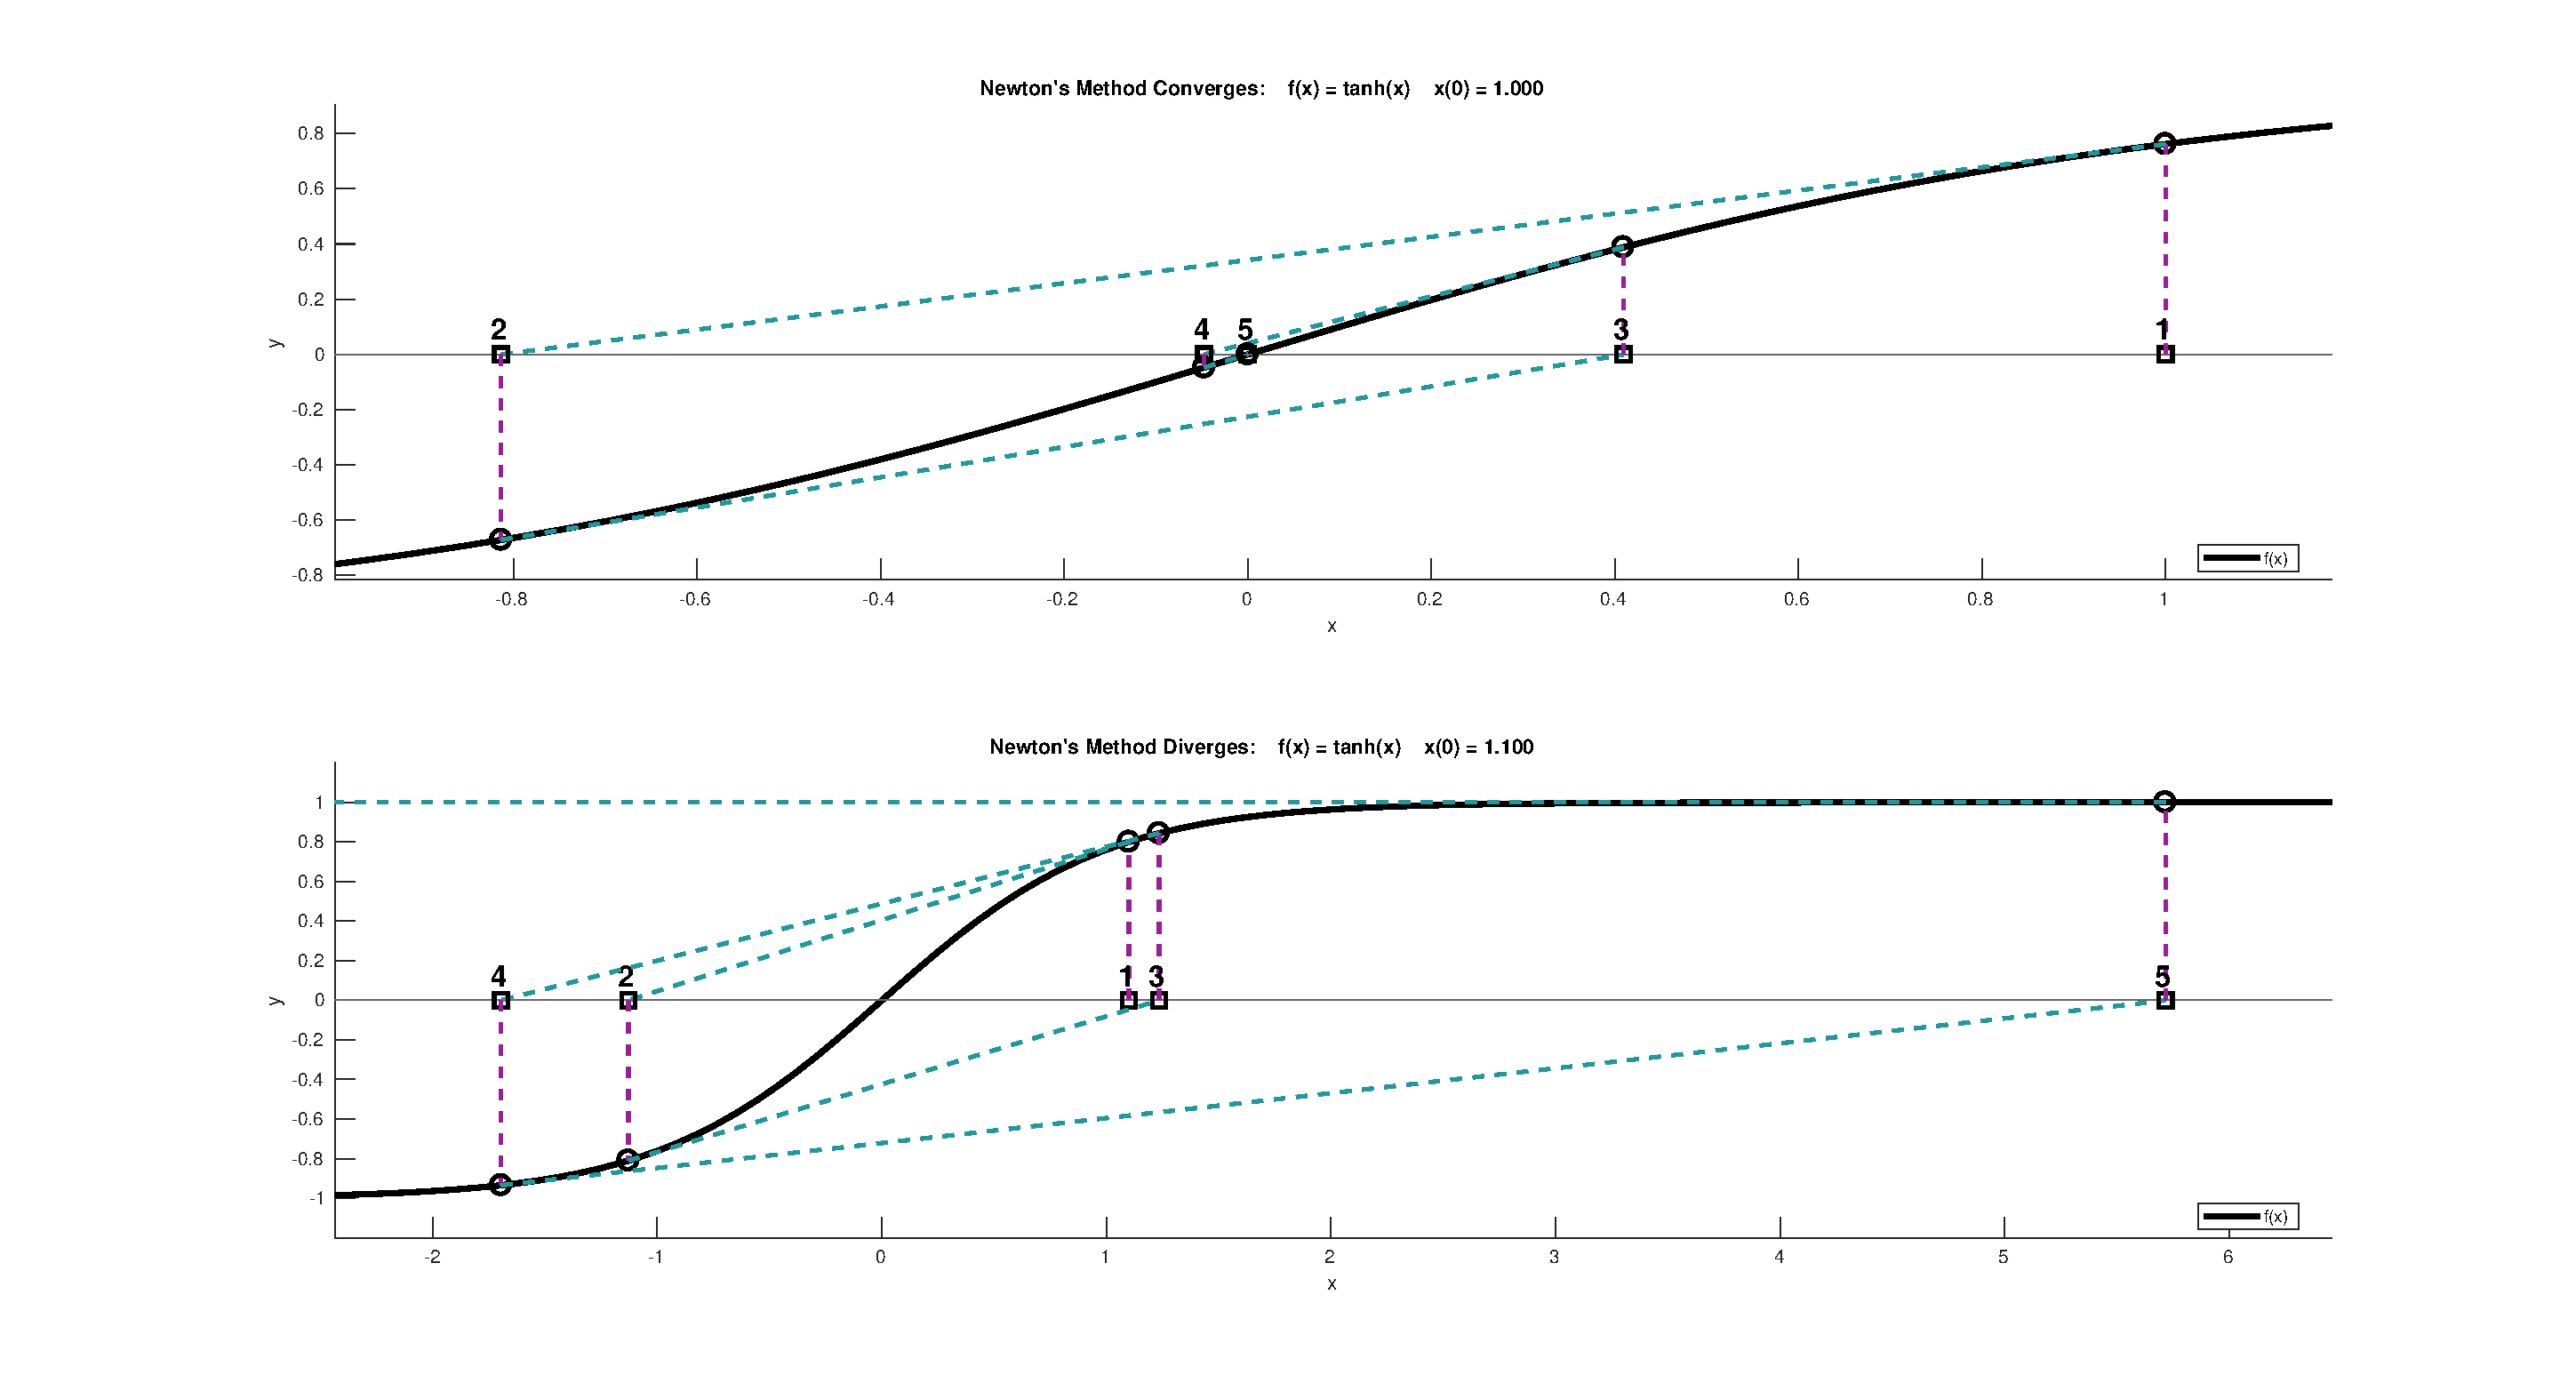
\includegraphics[width=\textwidth]{newtonRhapsonStability.pdf}
    \caption{Stability of Newton--Rhapson method for root finding}
    \label{fig:newtonRhapsonStability}
  \end{figure}

\end{enumerate}


%~~~~~~~~~~~~~~~~~~~~~~~~~~~~~~~~~~~~~~~~~~~~~~~~~~~~~~~~~~~~~~~~~~~~~~~~~~~~~

\section{Midpoint Method Implementation}

Implement the function \texttt{simStepMidpoint()} on the following page.
This function computes a single simulation step using the midpoint method.
You code should be clear, correct, and follow the best practices that
have been discussed throughout the course.
Use the space below for planning your solution.
Write your Matlab code inside of the function template on the following page.

\pagebreak
\lstset{stepnumber=0}
\lstinputlisting{simStepMidpoint.m}



\pagebreak
\section{Bisection Search}
\begin{NoHyper}
Use a bisection search to iteratively reduce the interval that is known
to bracket the root of the function shown in Figure \ref{fig:RootSolveExampleFigure}.
\textbf{Populate the table below}, showing the bracket for the first five iterations
and the new point that will be evaluated on that iteration.
\end{NoHyper}
\begin{itemize}  \setlength\itemsep{0.3em}
  \item \texttt{Iter 0:   bracket: [-1.000,  \hspace{2.7em}  1.000]  \hspace{1em}  xNew = 0.0}
  \item \texttt{Iter 1:   bracket: [-1.000,  \hspace{2.7em}  0.000]  \hspace{1em}  xNew = -0.5}
  \item \texttt{Iter 2:   bracket: [-0.500,  \hspace{2.7em}  0.000]  \hspace{1em}  xNew = -0.25}
  \item \texttt{Iter 3:   bracket: [-0.500,  \hspace{2.7em} -0.250]  \hspace{1em}  xNew = -0.375}
  \item \texttt{Iter 4:   bracket: [-0.375,  \hspace{2.7em} -0.250]  \hspace{1em}  xNew = -0.3125}
\end{itemize}

\begin{figure}[ht]
	\centering
  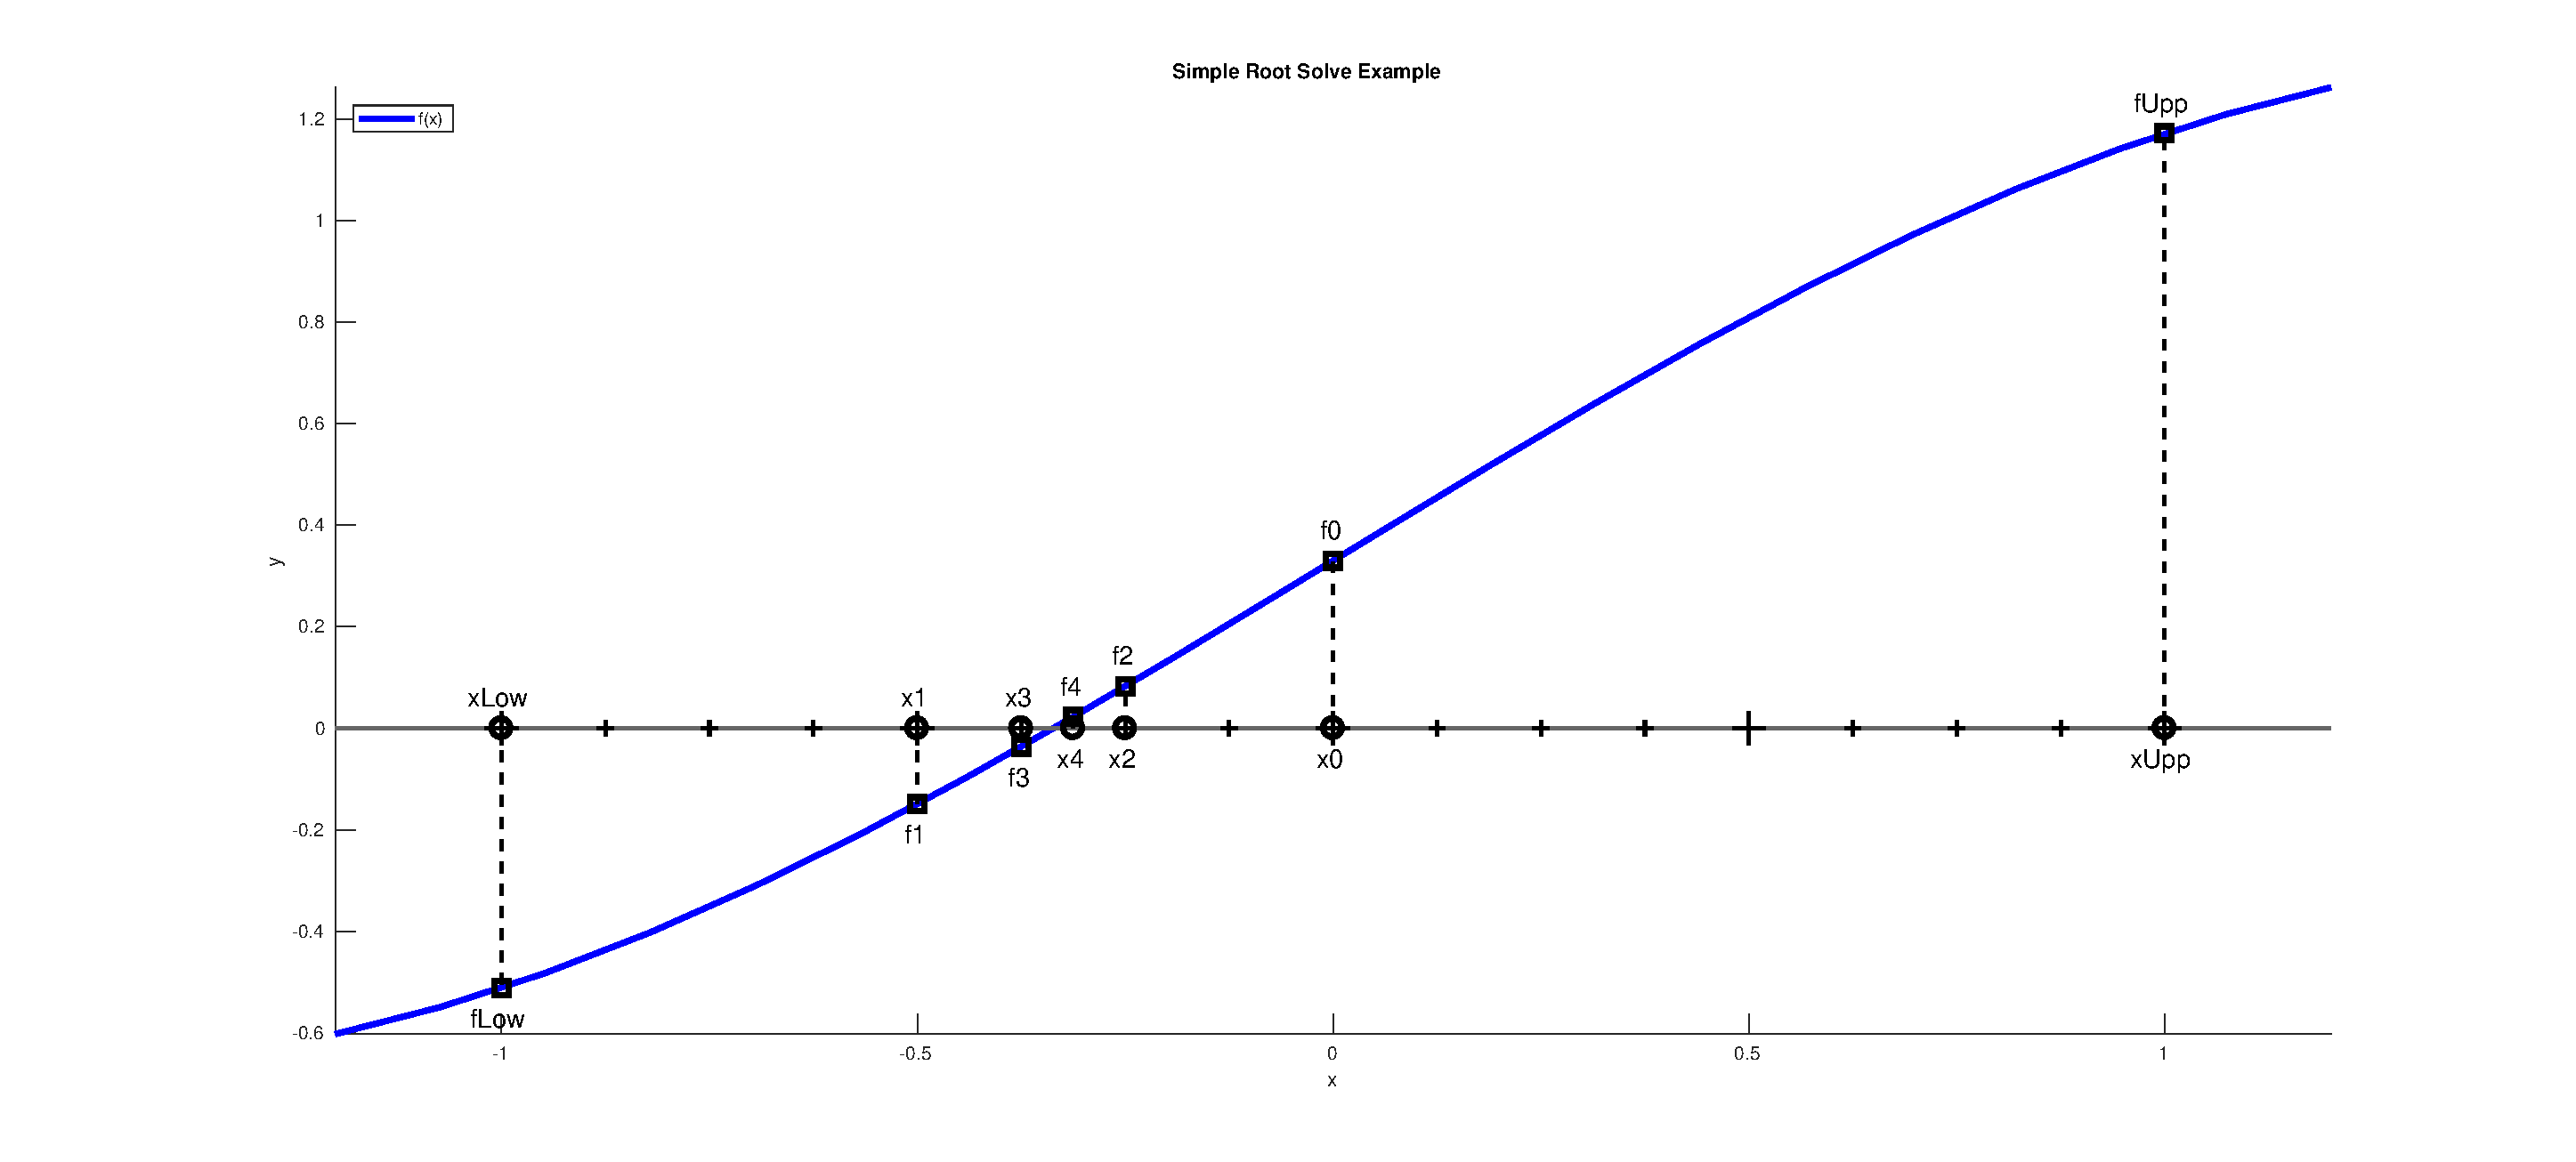
\includegraphics[width=\textwidth]{bisectionSearchFigure.pdf}
  \caption{Bisection Search Example Figure}
  \label{fig:RootSolveExampleFigure}
\end{figure}



%~~~~~~~~~~~~~~~~~~~~~~~~~~~~~~~~~~~~~~~~~~~~~~~~~~~~~~~~~~~~~~~~~~~~~~~~~~~~~

\pagebreak
\section{Scalar Taylor Series}

Write the Taylor series approximation of $f(t)$ to second-order around the point $t_0$.

\vspace{1em}
\begin{equation*}
  f(t) \approx f(t_0) + f'(t_0) \cdot (t - t_0) + f''(t_0) \cdot \tfrac{1}{2} (t - t_0)^2
\end{equation*}
\vspace{1em}
\begin{equation*}
  f'(t_0) = \frac{d}{dt} f(t) \big|_{t = t_0}
  \quad \quad \quad \quad
  f''(t_0) = \frac{d^2}{dt^2} f(t) \big|_{t = t_0}
\end{equation*}
\vspace{1em}

\section{Vector Taylor Series}

Write the Taylor series approximation of $f(t, \bm{x}, \bm{u})$ to first-order
about the point: $t_0$, $\bm{x}_0$, and $\bm{u}_0$.

\vspace{2em}
\begin{equation*}
  f(t, \bm{x}, \bm{u}) \approx
  f(t_0, \bm{x}_0, \bm{u}_0) +
  f_t(t_0, \bm{x}_0, \bm{u}_0) \cdot (t - t_0) +
  f_x(t_0, \bm{x}_0, \bm{u}_0) \cdot (\bm{x} - \bm{x}_0) +
  f_u(t_0, \bm{x}_0, \bm{u}_0) \cdot (\bm{u} - \bm{u}_0)
\end{equation*}
\vspace{1em}
\begin{equation*}
  f_t(t_0, \bm{x}_0, \bm{u}_0) = \frac{\delta}{\delta t} f(t, \bm{x}, \bm{u})
  \big|_{t = t_0, \bm{x} = \bm{x}_0, \bm{u} = \bm{u}_0}
\end{equation*}
\vspace{1em}
\begin{equation*}
  f_x(t_0, \bm{x}_0, \bm{u}_0) = \frac{\delta}{\delta x} f(t, \bm{x}, \bm{u})
  \big|_{t = t_0, \bm{x} = \bm{x}_0, \bm{u} = \bm{u}_0}
\end{equation*}
\vspace{1em}
\begin{equation*}
  f_u(t_0, \bm{x}_0, \bm{u}_0) = \frac{\delta}{\delta u} f(t, \bm{x}, \bm{u})
  \big|_{t = t_0, \bm{x} = \bm{x}_0, \bm{u} = \bm{u}_0}
\end{equation*}
\vspace{1em}

%~~~~~~~~~~~~~~~~~~~~~~~~~~~~~~~~~~~~~~~~~~~~~~~~~~~~~~~~~~~~~~~~~~~~~~~~~~~~~

\pagebreak
\section{Function Handle Gymnastics}
\textbf{What will the following script print out?} \\
For each part A, B, C, show your work and then box what will be printed.
\lstinputlisting{functionHandleGymnastics.m}

\subsection*{Part A:}
\texttt{A: 2}
\subsection*{Part B:}
\texttt{B: 12}
\subsection*{Part C: }
\texttt{C: 11}


%~~~~~~~~~~~~~~~~~~~~~~~~~~~~~~~~~~~~~~~~~~~~~~~~~~~~~~~~~~~~~~~~~~~~~~~~~~~~~

\pagebreak
\section{Matlab Programming Style}
The program below simulates a simple pendulum. It works, but is written poorly. \\
\textbf{Clearly identify at least 5 distinct issues with the code.}

\lstset{stepnumber=1}
\lstinputlisting{runSloppySimulation.m}

\begin{itemize}
  \item \textbf{Line 4:} arguments \texttt{@(t, z)} should be replaced with \texttt{@(\~ \,, z)}
  \item \textbf{Line 7:} plotting should include annotations
  \item \textbf{Line 17:} hard-coded time step --- should be a parameter
  \item \textbf{Line 11:} use \texttt{linspace} instead --- as written \texttt{tGrid(end)} is not \texttt{tUpp}
  \item \textbf{Line 12:} missing semicolon
  \item \textbf{Line 12-13:} as written, line 12 does nothing and line 13 allocates a matrix of the wrong size.
    These lines should be replaced by a correctly-written memory allocation
    and then setting the first column to the initial state.
  \item \textbf{Line 14:} \texttt{nDim} is unused --- this line should be deleted
  \item \textbf{Line 15:} upper loop limit should not be hard-coded
  \item \textbf{Line 16:} missing semicolon
  \item \textbf{Line 17:} hard-coded time step --- should be related to tGrid
\end{itemize}


%~~~~~~~~~~~~~~~~~~~~~~~~~~~~~~~~~~~~~~~~~~~~~~~~~~~~~~~~~~~~~~~~~~~~~~~~~~~~~


\pagebreak
\section{Linearized Dynamical System}

Given the non-linear system dynamics described below,

\begin{equation*}

  \dot{\bm{z}} =

  \begin{bmatrix}
    \dot{\alpha}  \\
    \dot{\gamma}  \\
    \dot{\theta}
  \end{bmatrix}

  =

  \begin{bmatrix}
    \beta \gamma + \theta^2 \\
    \alpha \, \sigma  - \theta\\
    \sin(\sigma) + \beta \, \gamma
  \end{bmatrix}

  = \bm{f}(\bm{z}, \bm{u})

  \quad \quad \quad \quad \quad \quad

  \bm{z} =
  \begin{bmatrix}
    \alpha \\
    \gamma \\
    \theta
  \end{bmatrix}

\quad \quad \quad \quad \quad \quad

  \bm{u} =
  \begin{bmatrix}
    \beta \\
    \sigma
  \end{bmatrix}


\end{equation*}



\vspace{0.5em}
\begin{enumerate}
  \item \textbf{List the state variables: } $\alpha, \; \gamma, \; \theta$
  \vspace{0.6em}
  \item \textbf{List the control variables: } $\beta, \; \sigma$
  \vspace{0.6em}
  \item \textbf{What is the difference between a state and a control variable? } \\
  \textit{State variables are those variables that have derivatives in the system dynamics.
          For example, both $\alpha$ and $\dot{\alpha}$ show up in the dynamics above.
          Control variables appear algebraically in the system dynamics.
          For example, $\sigma$ is in the system dynamics, but not $\dot{\sigma}$. }
  \item \textbf{Compute: } $\dfrac{\delta \bm{f}}{\delta \bm{z}}$

  \begin{equation*}
  \dfrac{\delta \bm{f}}{\delta \bm{z}} =
  \begin{bmatrix}
    0      & \beta & 2\theta \\
    \sigma & 0     & -1      \\
    0      & \beta & 0
  \end{bmatrix}
  \end{equation*}

  \item \textbf{Compute: } $\dfrac{\delta \bm{f}}{\delta \bm{u}}$

  \begin{equation*}
  \dfrac{\delta \bm{f}}{\delta \bm{u}} =
  \begin{bmatrix}
    \gamma & 0 \\
    0      & \alpha  \\
    \gamma & \cos{\sigma}
  \end{bmatrix}
  \end{equation*}


\end{enumerate}


%~~~~~~~~~~~~~~~~~~~~~~~~~~~~~~~~~~~~~~~~~~~~~~~~~~~~~~~~~~~~~~~~~~~~~~~~~~~~~
\pagebreak
\section{Trajectory Optimization}

Given the following continuous-time trajectory optimization problem.

\begin{align*}
  & \text{minimize: } \qquad J = \int_0^T \! g(t,\, \bm{x},\, \bm{u}) \, dt \\
  & \text{subject to: } \qquad \bm{0} = \bm{h}(\bm{x}(0), \, \bm{x}(T)) \\
  & \text{dynamics: } \qquad \dot{\bm{x}} = \bm{f}(t,\, \bm{x},\, \bm{u}) \\
\end{align*}

Suppose that you plan to solve the optimization using
direct multiple shooting with Euler's method
on a uniform grid of $N$ segments with one integration step per segment.
Write out the decision variables, objective function, and constraints
that will form the resulting non-linear program.

\begin{enumerate}
  \item \textbf{Decision Variables}
  \vspace{0.5em}
  \begin{equation*}
    \bm{x}_0, \bm{x}_1, \dots ,\bm{x}_N, \quad \bm{u}_0, \bm{u}_1, \dots, \bm{u}_{N-1}
  \end{equation*}
  \vspace{0.5em}
  \item \textbf{Objective Function}
  \vspace{0.5em}
  \begin{equation*}
    J = h \cdot \sum_{k=0}^{N-1} g(t_k,\,  \bm{x}_k,\,  \bm{u}_k)
  \end{equation*}
  \vspace{0.5em}
  \begin{equation*}
    h = \frac{T}{N}  \quad \quad \quad \quad t_k = k \cdot h
  \end{equation*}
  \vspace{0.5em}
  \item \textbf{Boundary Constraints}
  \vspace{0.5em}
  \begin{equation*}
    \bm{0} = \bm{h}(\bm{x}_0, \, \bm{x}_N)
  \end{equation*}
  \vspace{0.5em}
  \item \textbf{System Dynamics Constraints}
  \vspace{0.5em}
  \begin{equation*}
    \bm{x}_{k+1} = \bm{x}_k + h \cdot \bm{f}(t_k,\, \bm{x}_k,\, \bm{u}_k)
    \quad \quad k \in 0 \dots (N-1)
  \end{equation*}
  \vspace{0.5em}
\end{enumerate}

%=================================================
\end{document}
